%!TEX root=../main.tex
\section{More results} % (fold)
\label{sec:more_results}


\subsection{Simulation} % (fold)
\label{sub:simulation}

We present the results of the simulations in the sparse and noisy cases. Figures \ref{fig:logAE_mfd_1d_noise}, \ref{fig:ise_mfd_1d_noise} and \ref{fig:mise_mfd_1d_noise} present the boxplots of the RSE, ISE and MRSE, respectively, for the noisy case. To generate noisy data, we consider the model \eqref{eq:model_error} where $\sigma^2 = 0.25$. For the \texttt{(Tensor) PCA} method, we first smooth the 2-dimensional data using P-Splines smoothing and estimate a smooth version of the mean and covariance functions for the one-dimensional data using P-Splines smoothing. For the \texttt{2D/1D B-Splines} and \texttt{Gram} methods, all the observations have been smoothed using P-Splines smoothing beforehand. In every case, the penalty involved in P-Splines smoothing has been estimated using cross-validation.

\begin{figure}
    \centering
    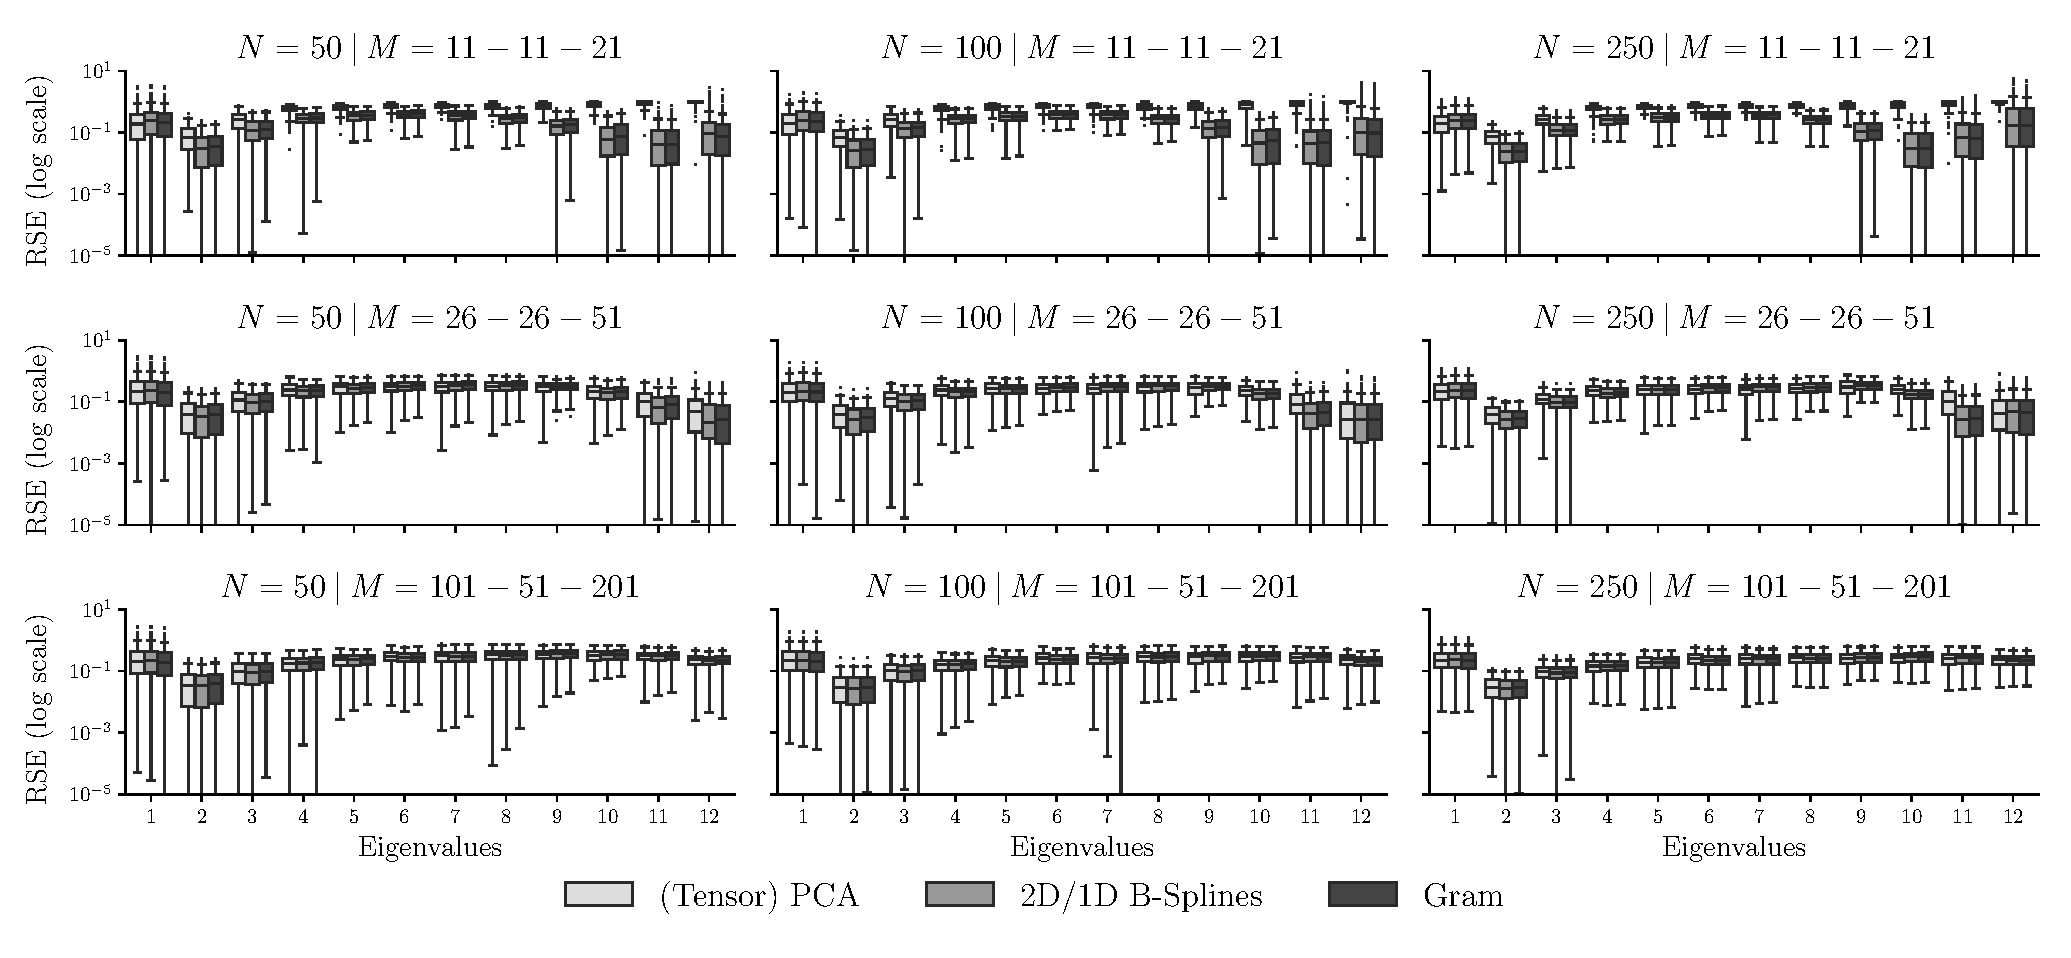
\includegraphics[width=0.95\textwidth]{figures/AE_noise.eps}
    \caption{RSE for the estimated eigenvalues for each method in the noisy case. $N$ is the number of observations, $M$ is the number of sampling points per curve (the first two numbers are for the images and the last one is for the curves).}
    \label{fig:logAE_mfd_1d_noise}
\end{figure}

\begin{figure}
    \centering
    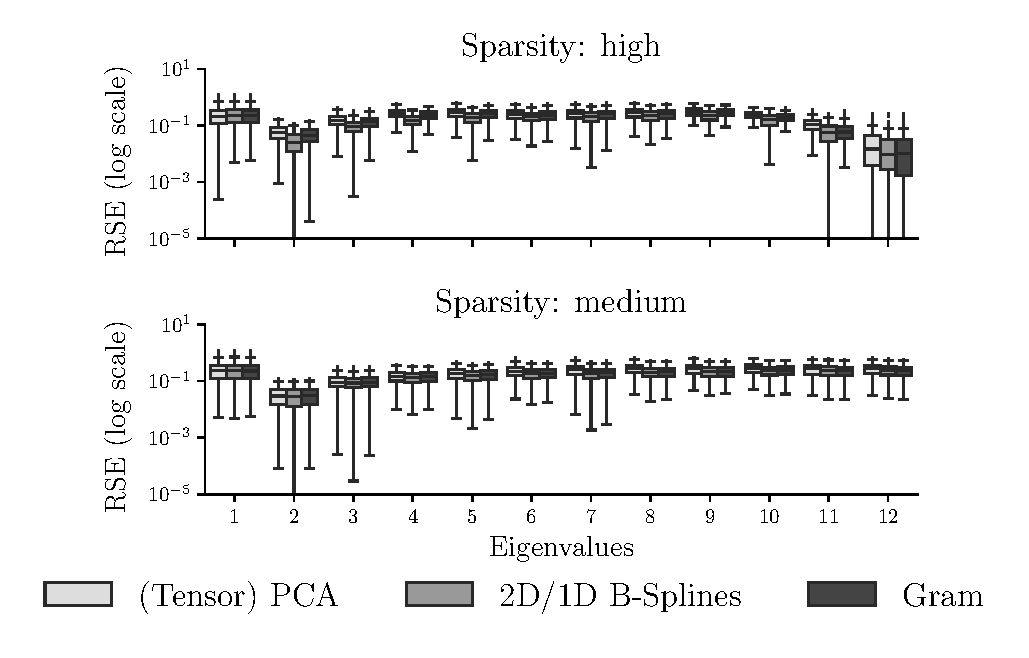
\includegraphics[width=0.8\textwidth]{figures/AE_sparse.eps}
    \caption{RSE for the estimated eigenvalues for each method in the sparse case. We set $N = 250$, $M^{(1)} = 101 \times 51$ and $M^{(2)} = 201$. For the case of medium sparsity, we remove $50\%-70\%$ of the sampling points and for the case of high sparsity, we remove $90\%-95\%$ of the sampling points.}
    \label{fig:logAE_mfd_1d_sparse}
\end{figure}


Figures \ref{fig:logAE_mfd_1d_sparse}, \ref{fig:ise_mfd_1d_sparse} and \ref{fig:mise_mfd_1d_sparse} present the boxplots of the RSE, ISE and MRSE, respectively, for the sparse case. In this case, we only consider $N = 250$, $M^{(1)} = 101 \times 51$, $M^{(2)} = 201$ and no noise. We consider medium sparsity, where $50\%-70\%$ of the sampling points have been removed and high sparsity, where $90\%-95\%$ of the sampling points have been removed. For the \texttt{(Tensor) PCA} method, we first interpolate the 2-dimensional data to have the observations reguarlarly sampled on a grid and estimate a smooth version of the mean and covariance functions for the one-dimensional data using P-Splines smoothing. For the \texttt{2D/1D B-Splines} method, all the observations have been smoothed using P-splines smoothing with a penalty estimated by cross-validation. For the \texttt{Gram} method, the observations have been linearly interpolated to estimate the inner-product matrix.



\begin{figure}
     \centering
    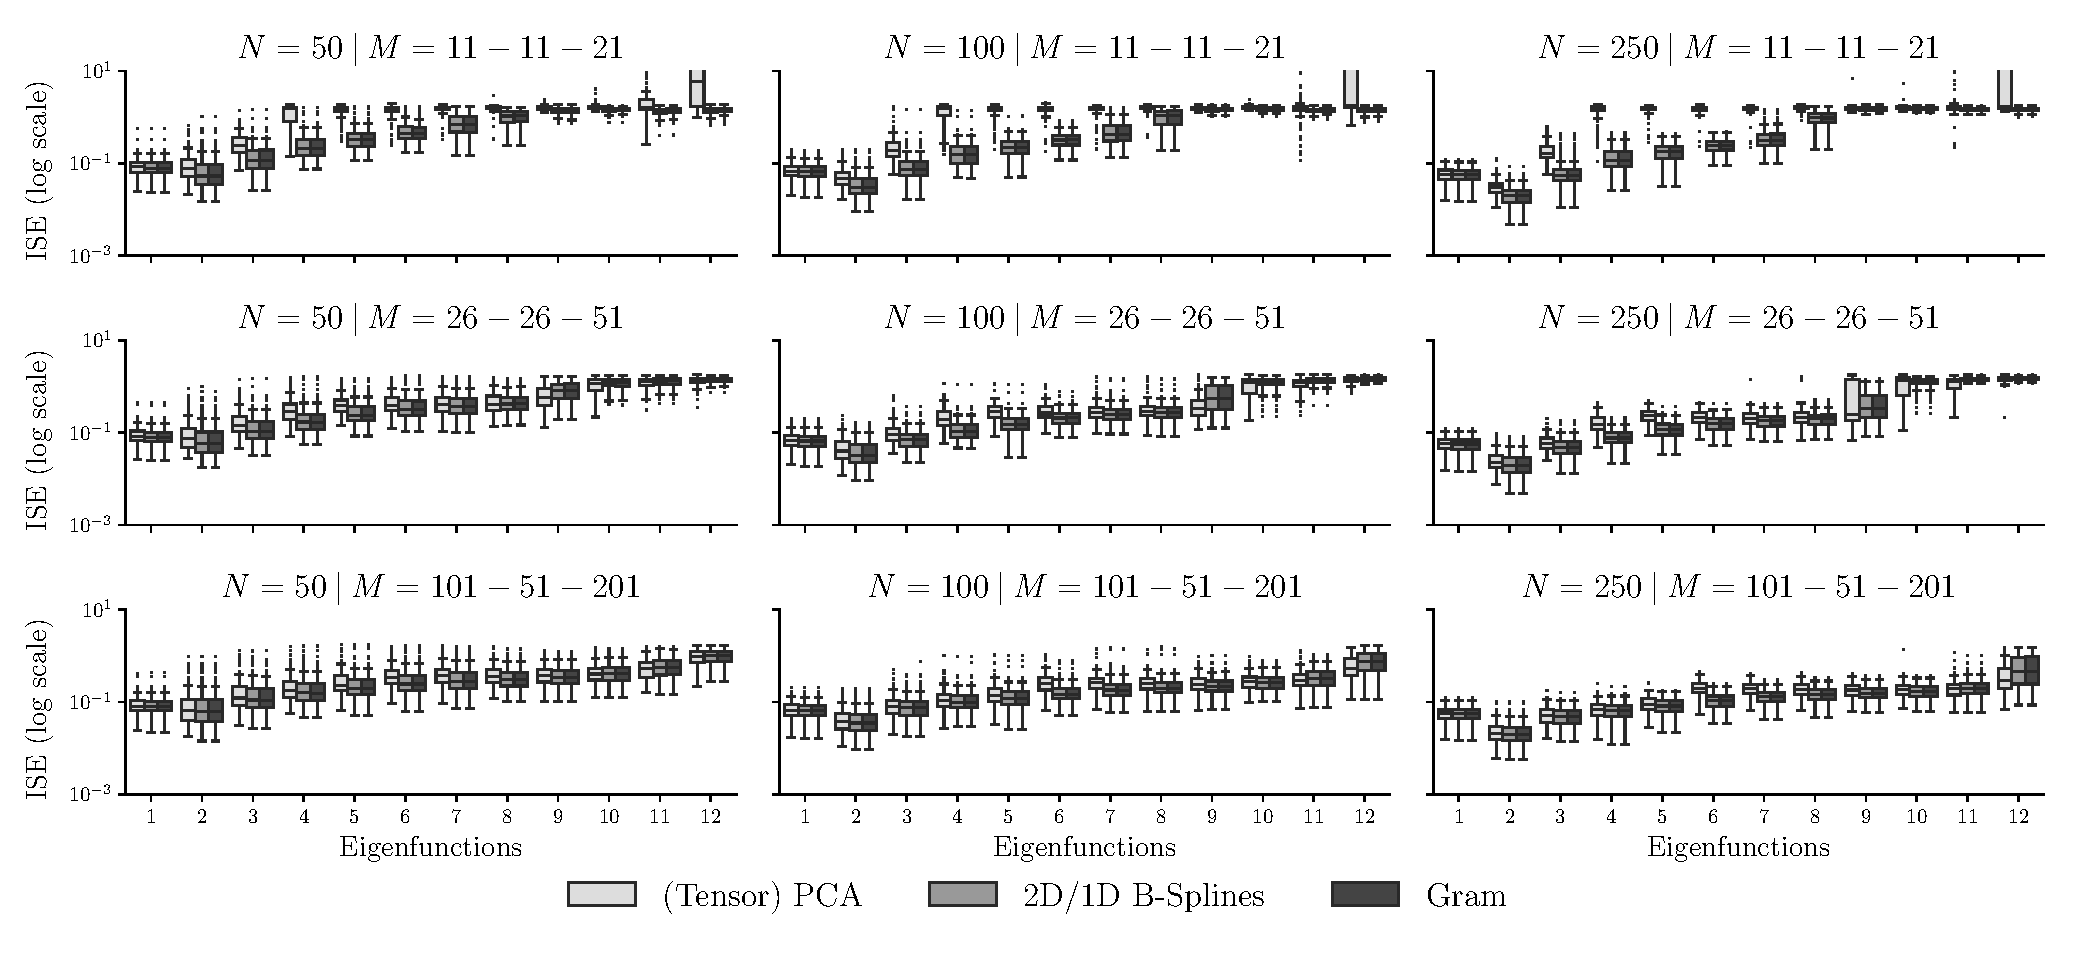
\includegraphics[width=0.95\textwidth]{figures/ISE_noise.eps}
    \caption{ISE for the estimated eigenfunctions for each method in the noisy case. $N$ is the number of observations, $M$ is the number of sampling points per curve (the first two numbers are for the images and the last one is for the curves).}
    \label{fig:ise_mfd_1d_noise}
\end{figure}

\begin{figure}
     \centering
    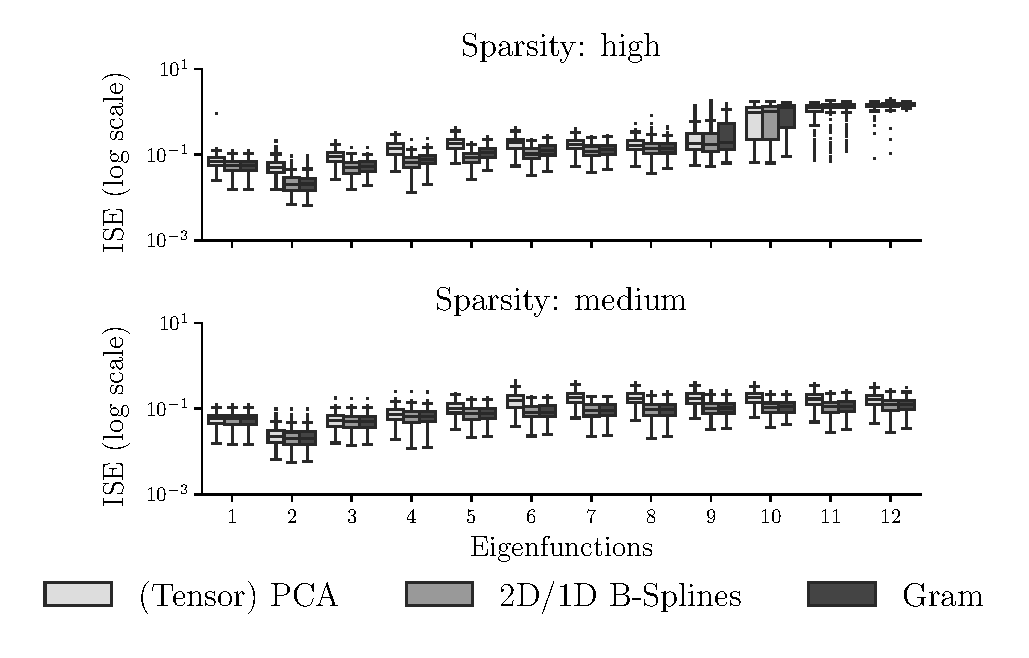
\includegraphics[width=0.95\textwidth]{figures/ISE_sparse.eps}
    \caption{ISE for the estimated eigenfunctions for each method in the sparse case. We set $N = 250$, $M^{(1)} = 101 \times 51$ and $M^{(2)} = 201$. For the case of medium sparsity, we remove $50\%-70\%$ of the sampling points and for the case of high sparsity, we remove $90\%-95\%$ of the sampling points.}
    \label{fig:ise_mfd_1d_sparse}
\end{figure}


\begin{figure}
     \centering
     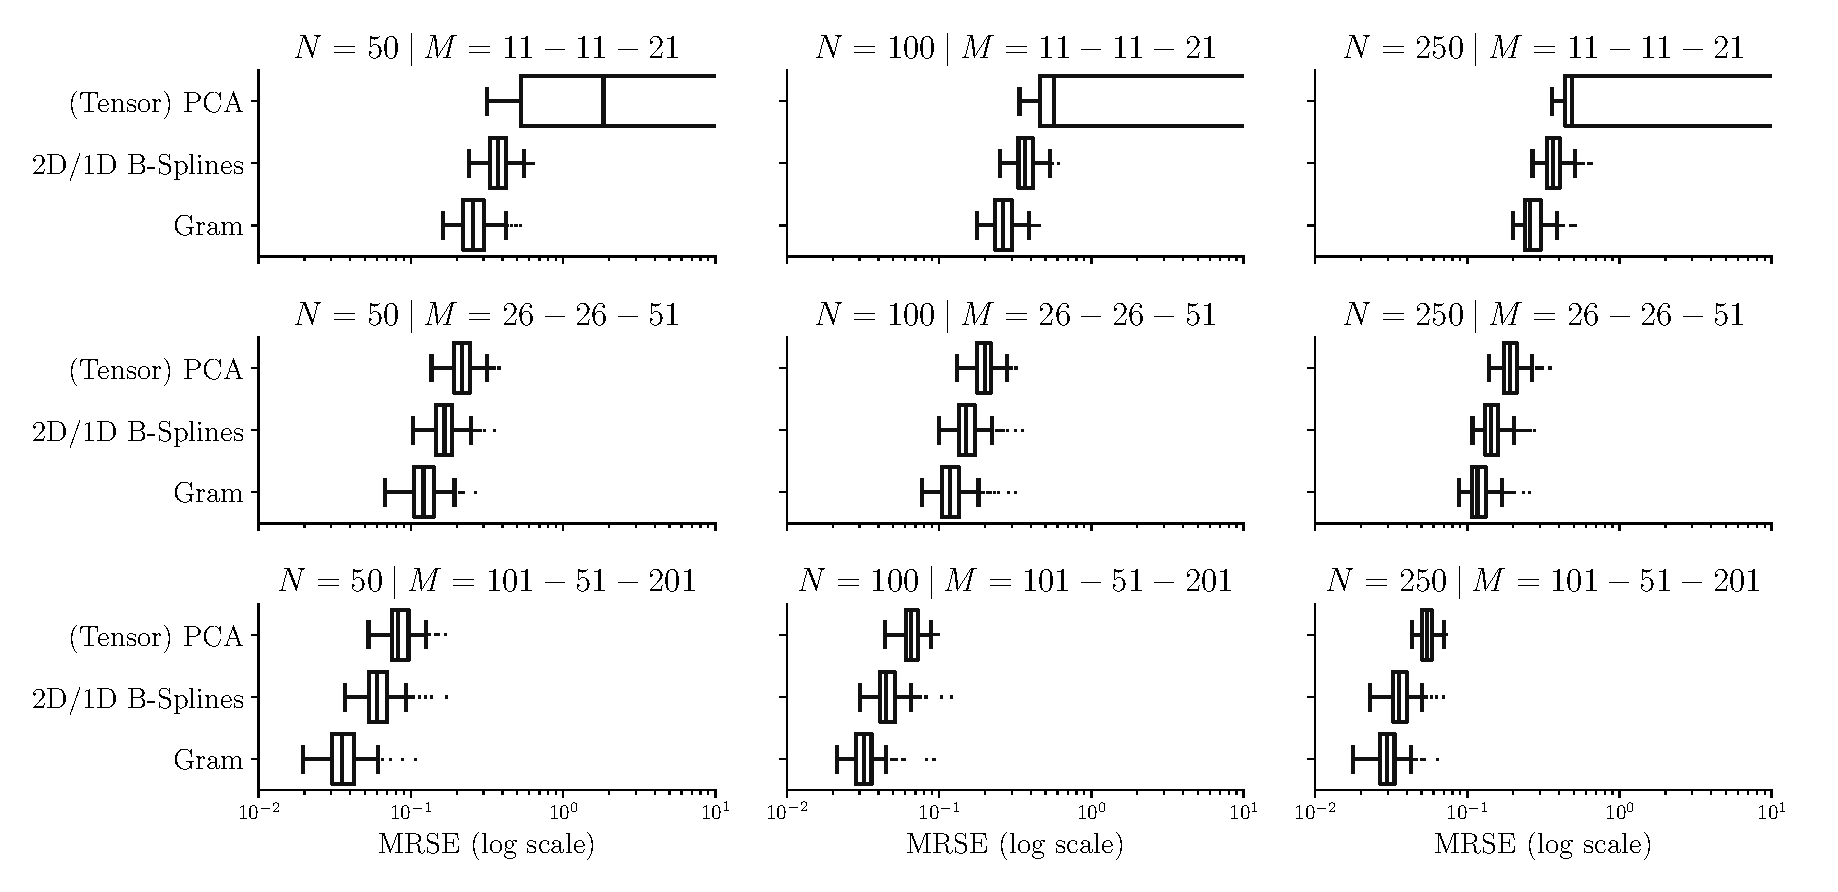
\includegraphics[width=0.95\textwidth]{figures/MRSE_noise.eps}
    \caption{MRSE for the reconstructed curves for each method in the noisy case. $N$ is the number of observations, $M$ is the number of sampling points per curve (the first two numbers are for the images and the last one is for the curves).}
    \label{fig:mise_mfd_1d_noise}
\end{figure}

\begin{figure}
     \centering
     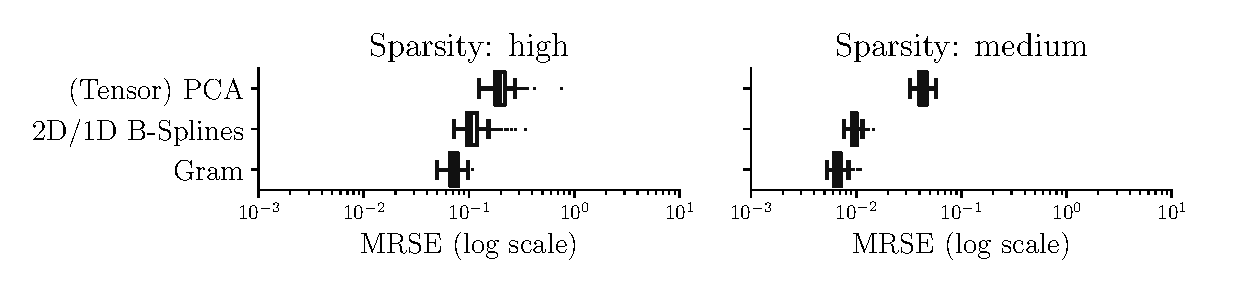
\includegraphics[width=0.95\textwidth]{figures/MRSE_sparse.eps}
    \caption{MRSE for the reconstructed curves for each method in the sparse case. We set $N = 250$, $M^{(1)} = 101 \times 51$ and $M^{(2)} = 201$. For the case of medium sparsity, we remove $50\%-70\%$ of the sampling points and for the case of high sparsity, we remove $90\%-95\%$ of the sampling points.}
    \label{fig:mise_mfd_1d_sparse}
\end{figure}

% subsection simulation (end)

\subsection{Application} % (fold)
\label{sub:application}

Here, we present the estimation of the eigencomponents of the shooting data using the \texttt{(Tensor) PCA} (see Figure~\ref{fig:eigenfunctions_fcptpa}) and \texttt{2D/1D B-Splines} (see Figure~\ref{fig:eigenfunctions_psplines}) methods. The results are similar to those found using the \texttt{Gram} method for the eigenfunctions and the percentage of variance explained for each eigenfunctions.

\begin{figure}
    \centering
    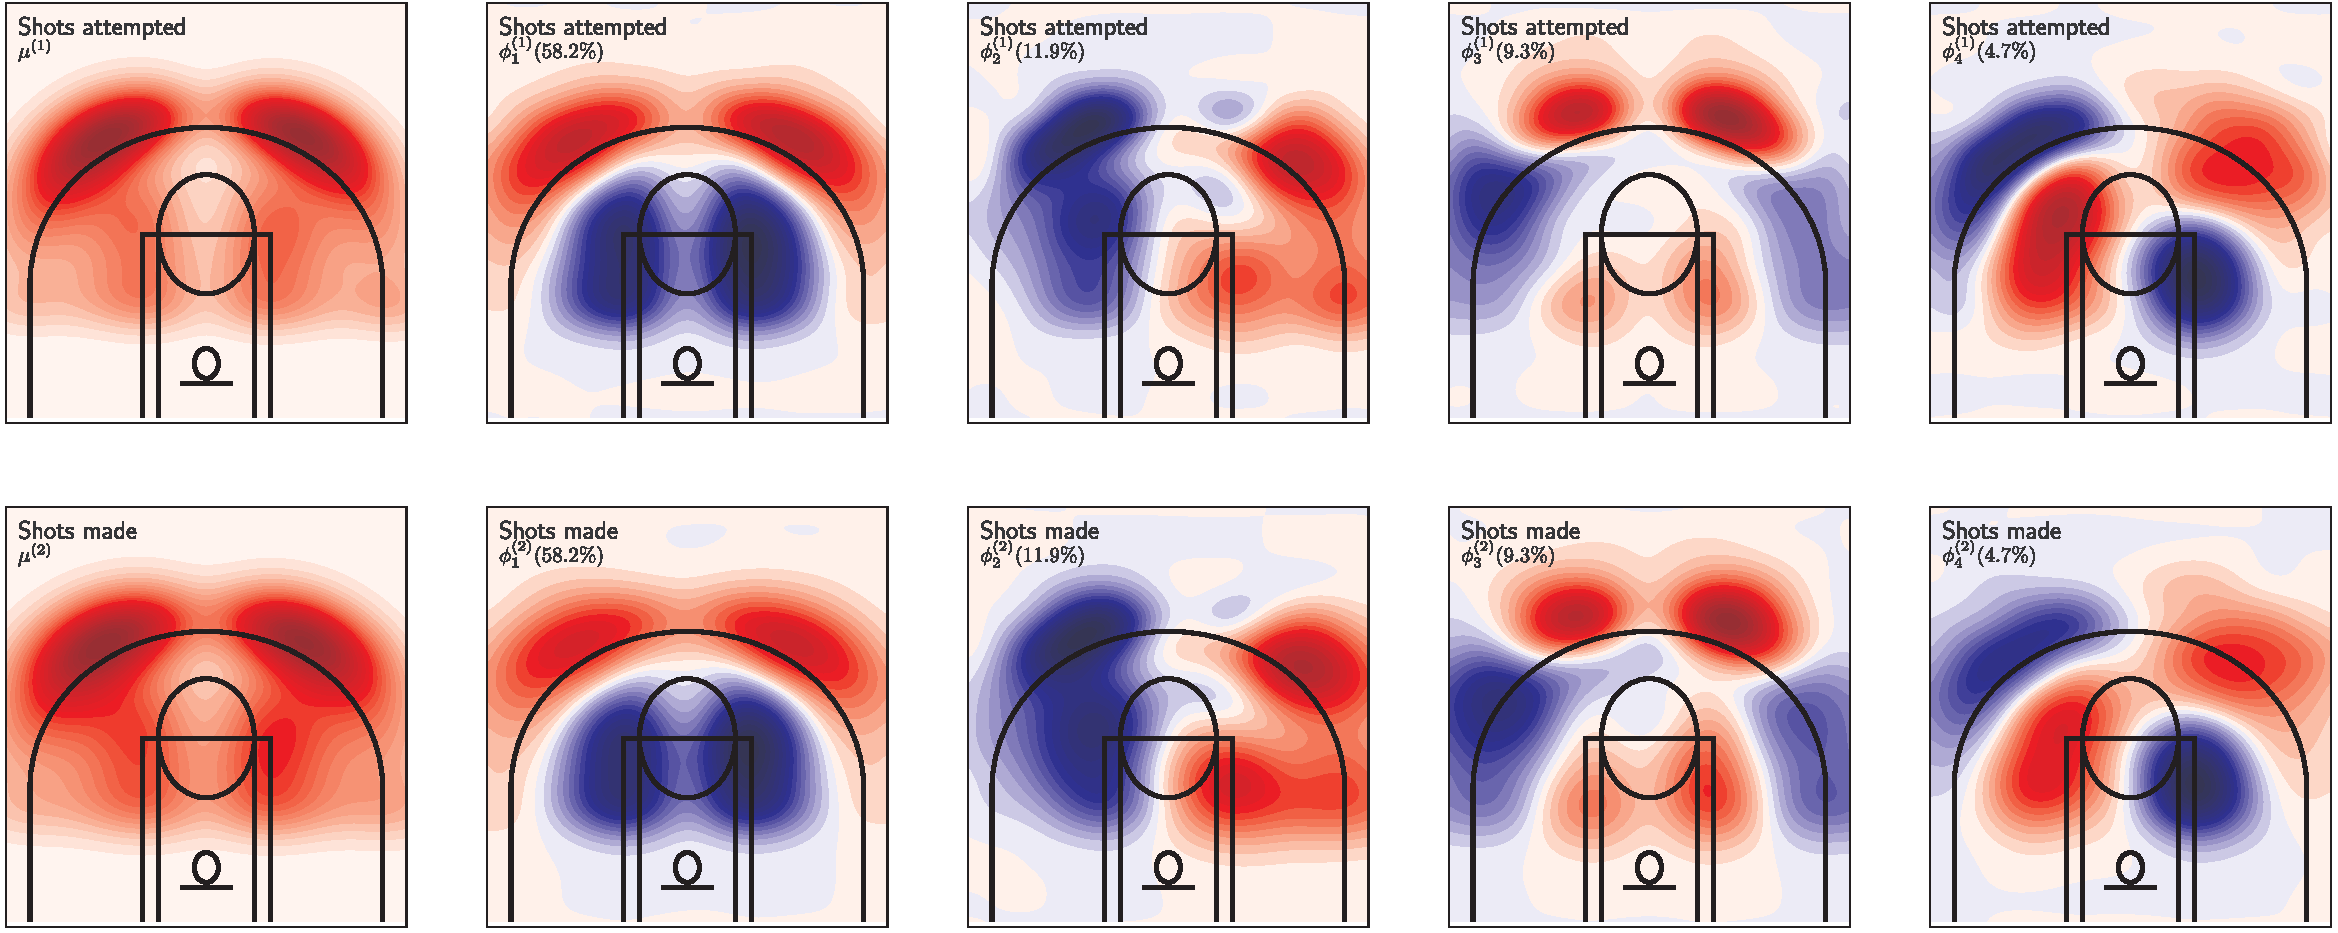
\includegraphics[width=\textwidth]{figures/eigenfunctions_fcptpa.eps}
    \caption{The estimated mean surfaces (first column) and the estimated eigenfunctions (second to fifth columns) for the shots dataset using the \texttt{(Tensor) PCA} method.}
    \label{fig:eigenfunctions_fcptpa}
\end{figure}

\begin{figure}
    \centering
    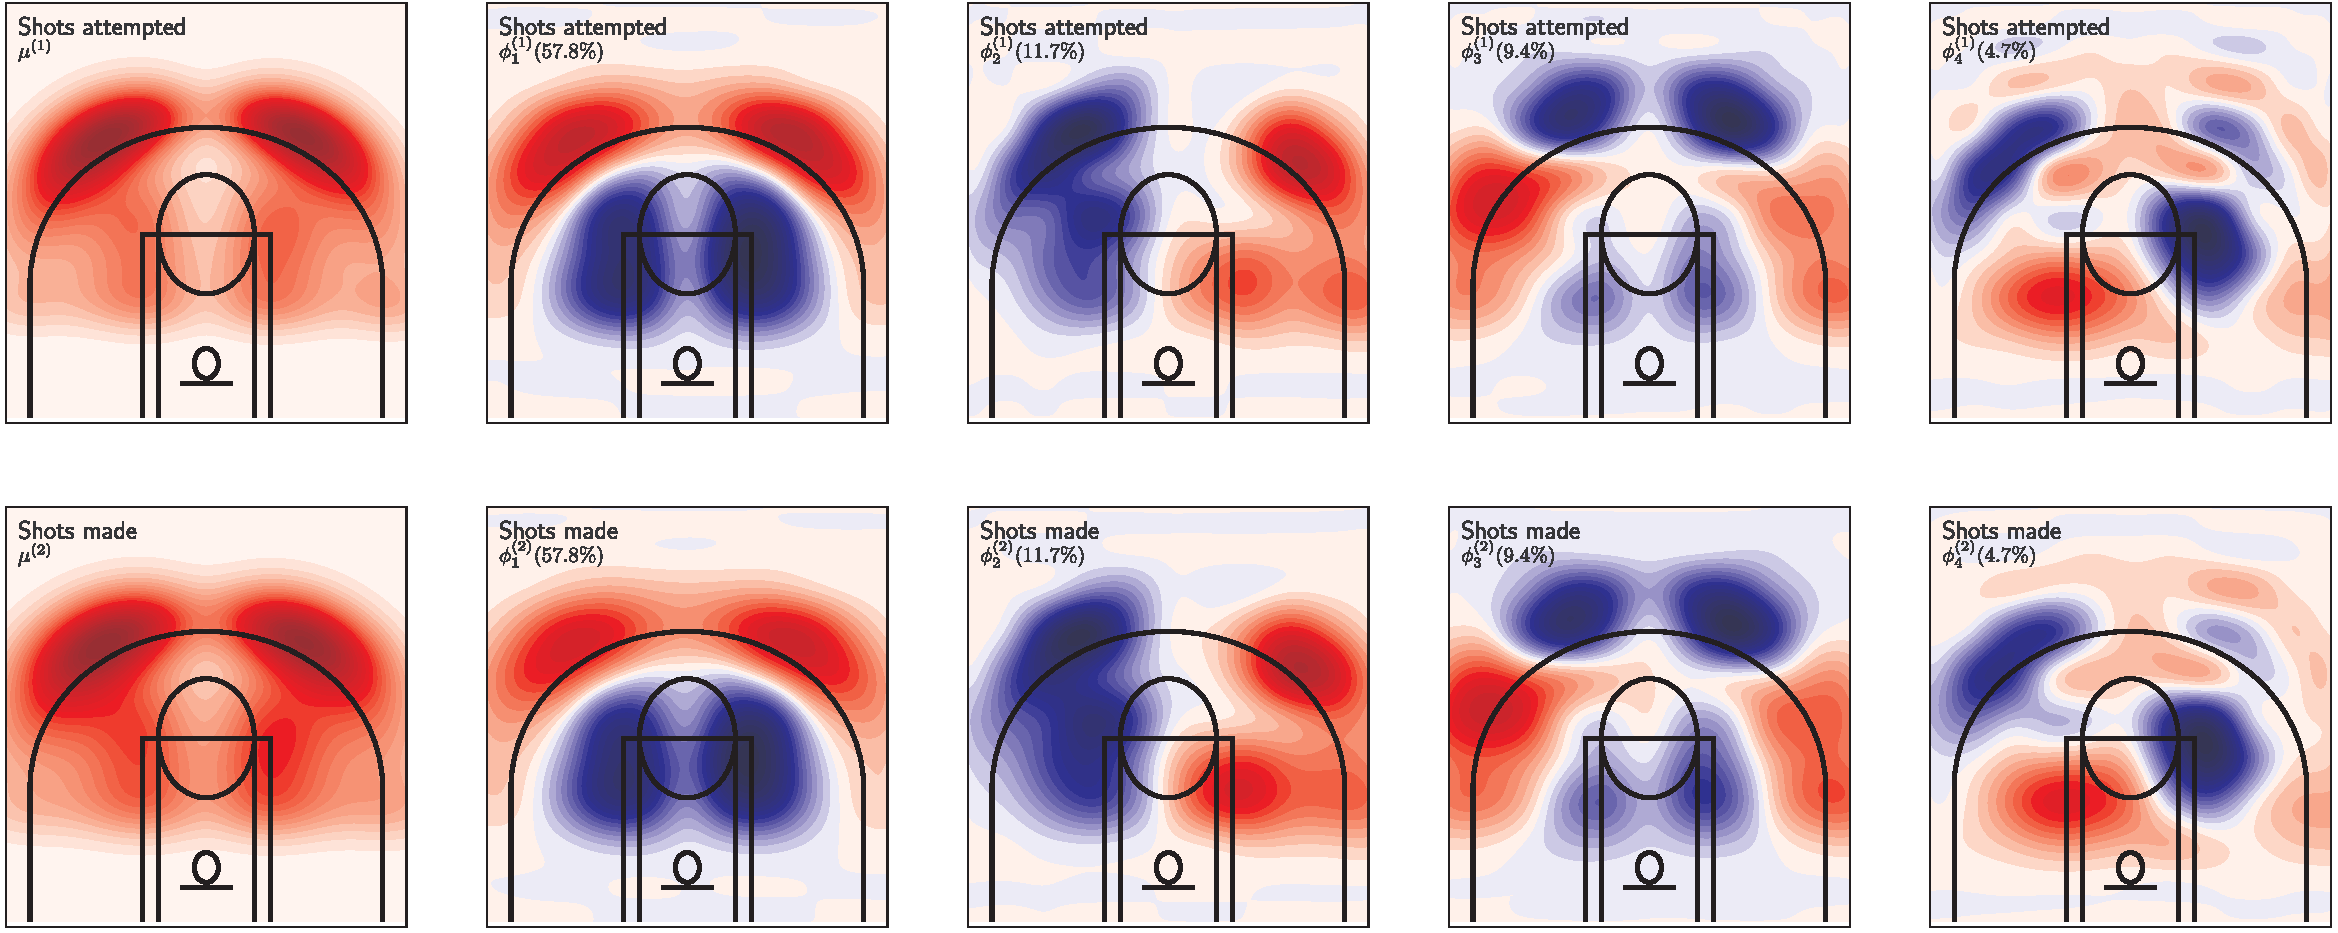
\includegraphics[width=\textwidth]{figures/eigenfunctions_psplines.eps}
    \caption{The estimated mean surfaces (first column) and the estimated eigenfunctions (second to fifth columns) for the shots dataset using the \texttt{2D/1D B-splines} method.}
    \label{fig:eigenfunctions_psplines}
\end{figure}

% subsection application (end)

% section more_results (end)